% \documentclass[aspectratio=169,notes]{beamer}
\documentclass[aspectratio=169]{beamer}
\usetheme[faculty=phil]{fibeamer}
\usepackage{polyglossia}
\setmainlanguage{english} %% main locale instead of `english`, you
%% can typeset the presentation in either Czech or Slovak,
%% respectively.
\setotherlanguages{russian} %% The additional keys allow
%%
%%   \begin{otherlanguage}{czech}   ... \end{otherlanguage}
%%   \begin{otherlanguage}{slovak}  ... \end{otherlanguage}
%%
%% These macros specify information about the presentation
\title[Artificial Intelligence Software (AIS)]{Artificial Intelligence Software, Lecture 3} %% that will be typeset on the
\subtitle{AI Paper Pipeline: Writing, Reading, and Reviewing with AI 
\\ \ \\ \  } %% title page.
\author{Oleg Bulichev}
%% These additional packages are used within the document:
\usepackage{ragged2e}  % `\justifying` text
\usepackage{booktabs}  % Tables
\usepackage{tabularx}
\usepackage{tikz}      % Diagrams
\usetikzlibrary{calc, shapes, backgrounds, trees, positioning, arrows.meta}
\usetikzlibrary{decorations.pathreplacing,calligraphy,calc,graphs}
\usepackage{amsmath, amssymb}
\usepackage{url}       % `\url`s
\usepackage{listings}  % Code listings
\usepackage{floatrow}
\usepackage{subcaption}
\usepackage{mathtools}
\usepackage{todonotes}
\usepackage{fontspec}
\usepackage{multicol}
\usepackage{pdfpages}
\usepackage{wrapfig}
\usepackage{qrcode}
\usepackage{animate}
\usepackage{booktabs}
\usepackage{multirow}
\usepackage{graphicx}
\usepackage{colortbl}

\graphicspath{{resources/}}
\frenchspacing

\setbeamertemplate{caption}{\raggedright\insertcaption\par}
\usetikzlibrary{graphs}

% \usepackage[backend=biber,style=ieee,autocite=footnote]{biblatex}
% \addbibresource{biblio.bib}
% \DefineBibliographyStrings{english}{%
%   bibliography = {References},}

\newcommand{\oleg}[2][] {\todo[color=red, #1] {OLEG:\\ #2}}
\newcommand{\fbckg}[1]{\usebackgroundtemplate{\includegraphics[width=\paperwidth]{#1}}}%frame background

\usepackage[framemethod=TikZ]{mdframed}
\newcommand{\dbox}[1]{
\begin{mdframed}[roundcorner=3pt, backgroundcolor=yellow, linewidth=0]
\vspace{1mm}
{#1}
\vspace{1mm}
\end{mdframed}
}

\begin{document}
\setlength{\abovedisplayskip}{0pt}
\setlength{\belowdisplayskip}{0pt}
\setlength{\abovedisplayshortskip}{0pt}
\setlength{\belowdisplayshortskip}{0pt}

\fbckg{fibeamer/figs/title_page.png}
\frame[c]{\setcounter{framenumber}{0}
    \usebeamerfont{title}%
    \usebeamercolor[fg]{title}%
    \begin{minipage}[b][6.5\baselineskip][b]{\textwidth}%
        \textcolor{black}{\raggedright\inserttitle}
    \end{minipage}
    % \vskip-1.5\baselineskip

    \usebeamerfont{subtitle}%
    \usebeamercolor[fg]{framesubtitle}%
    \begin{minipage}[b][3\baselineskip][b]{\textwidth}
        \raggedright%
        \insertsubtitle%
    \end{minipage}
    \vskip.25\baselineskip
}

\fbckg{fibeamer/figs/common.png}

\begin{frame}[t]{Outline}
    \vspace*{-1cm}
    \begin{columns}[t]
        
        \begin{column}{0.5\textwidth}
            \tableofcontents[sections={1-5}, hideallsubsections]
        \end{column}
        \begin{column}{0.5\textwidth}
            \tableofcontents[sections={6-}, hideallsubsections]
        \end{column}
    \end{columns}
\end{frame}

\section{Introduction}

\begin{frame}[t]{Introduction: The Researcher in the AI Era}
    \begin{itemize}
        \item \textbf{Role Shift:} From generating text to generating meaning. AI is a tool, not the author.
        \item \textbf{Knowledge vs. Data:} AI models reflect existing ideas. New knowledge comes from researchers.
        \item \textbf{The Noise Problem:}
        \begin{itemize}
            \item Easier to generate text $\to$ Flood of low-quality papers.
            \item Speed vs. Quality trade-off.
        \end{itemize}
        \item \textbf{Value of True Research:} High-quality, reproducible work stands out more than ever.
    \end{itemize}
\end{frame}

\begin{frame}[t]{Publish or Perish: New Reality}
    \begin{columns}
        \begin{column}{0.5\textwidth}
            \begin{tikzpicture}[scale=0.8]
                % Axes
                \draw[->] (0,0) -- (5,0) node[right] {Time};
                \draw[->] (0,0) -- (0,4) node[above] {Quantity};
                
                % Exponential growth of papers (red)
                \draw[red, thick, domain=0:4.5] plot (\x, {0.2*exp(\x*0.7)});
                \node[red] at (2.0, 3.5) {AI-generated noise};
                
                % Linear growth of quality (blue)
                \draw[blue, thick, domain=0:4.5] plot (\x, {0.5 + 0.3*\x});
                \node[blue] at (4.5, 1.0) {True breakthroughs};
                
                % Gap
                \draw[<->, dashed] (4, 3.2) -- (4, 1.7); 
                \node[right, align=left, font=\scriptsize] at (4.1, 2.5) {The Gap:\\ Need for filtering};
            \end{tikzpicture}
        \end{column}
        \begin{column}{0.5\textwidth}
            \begin{itemize}
                \item \textbf{Reproducibility} is the new competitive advantage.
                \item \textbf{Open Code} is a sign of respect.
                \item \textbf{Transparency} builds trust.
            \end{itemize}
        \end{column}
    \end{columns}
\end{frame}

\begin{frame}[t]{Responsibility and Reputation}
    \begin{itemize}
        \item \textbf{Author's Responsibility:}
        \begin{itemize}
            \item Setting the research problem.
            \item Conducting experiments.
            \item Interpreting results.
            \item Ethics and safety.
        \end{itemize}
        \item \textbf{Reputation:} AI can write, but it cannot own the results.
        \item \textbf{Expertise:} You are the navigator in the information noise.
    \end{itemize}
\end{frame}


\section{Lifecycle of a Paper}

\begin{frame}[t]{Paper Lifecycle Overview}
\vspace*{-0.5cm}
\begin{figure}[H]
    \centering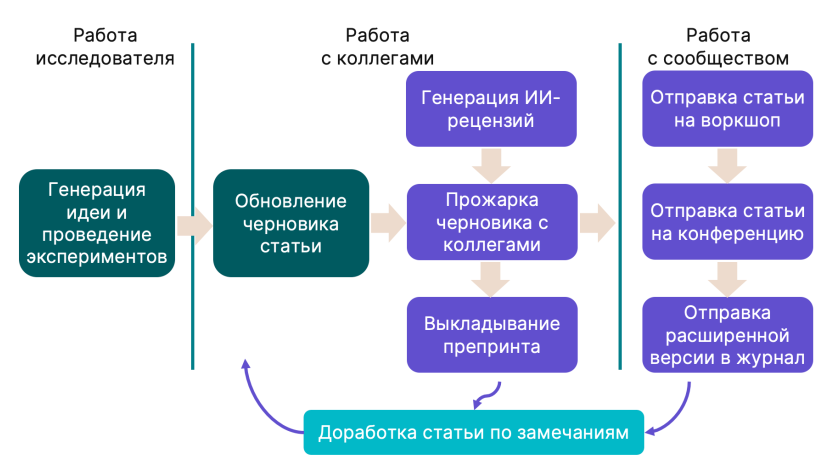
\includegraphics[height=6cm,width=1\textwidth,keepaspectratio]{2_1.png}
    % \caption{caption_name}
    \label{fig:2_1.png}
\end{figure}
\end{frame}

\begin{frame}[t]{The Process Levels}
    \begin{enumerate}
        \item \textbf{Researcher's Work:}
        \begin{itemize}
            \item Idea generation \& Experiments.
            \item Drafting (iterative process).
        \end{itemize}
        \item \textbf{Collaborative Work:}
        \begin{itemize}
            \item Internal review (Colleagues).
            \item AI pre-review (sanity check).
        \end{itemize}
        \item \textbf{Community Work:}
        \begin{itemize}
            \item Submission (Conferences, Workshops, Journals).
            \item External Review \& Rebuttal.
        \end{itemize}
    \end{enumerate}
\end{frame}

\begin{frame}[t]{Preparation for Submission}
    \begin{itemize}
        \item \textbf{Deadlines:} Planning is key (Abstract deadline vs Full paper deadline).
        \item \textbf{Venue Selection:} ICLR, NeurIPS, ICML, CVPR, AAAI, etc.
        \item \textbf{Formal Requirements:}
        \begin{itemize}
            \item Page limits (Strict!).
            \item Templates (LaTeX).
            \item Anonymity (Double-blind review).
        \end{itemize}
    \end{itemize}
\end{frame}

\begin{frame}[t]{Submission Systems}
    \begin{columns}
        \begin{column}{0.5\textwidth}
            \textbf{OpenReview.net} (ICLR, NeurIPS)
            \begin{center}
                \begin{minipage}{0.9\textwidth}
                    \begin{figure}[H]
                        \centering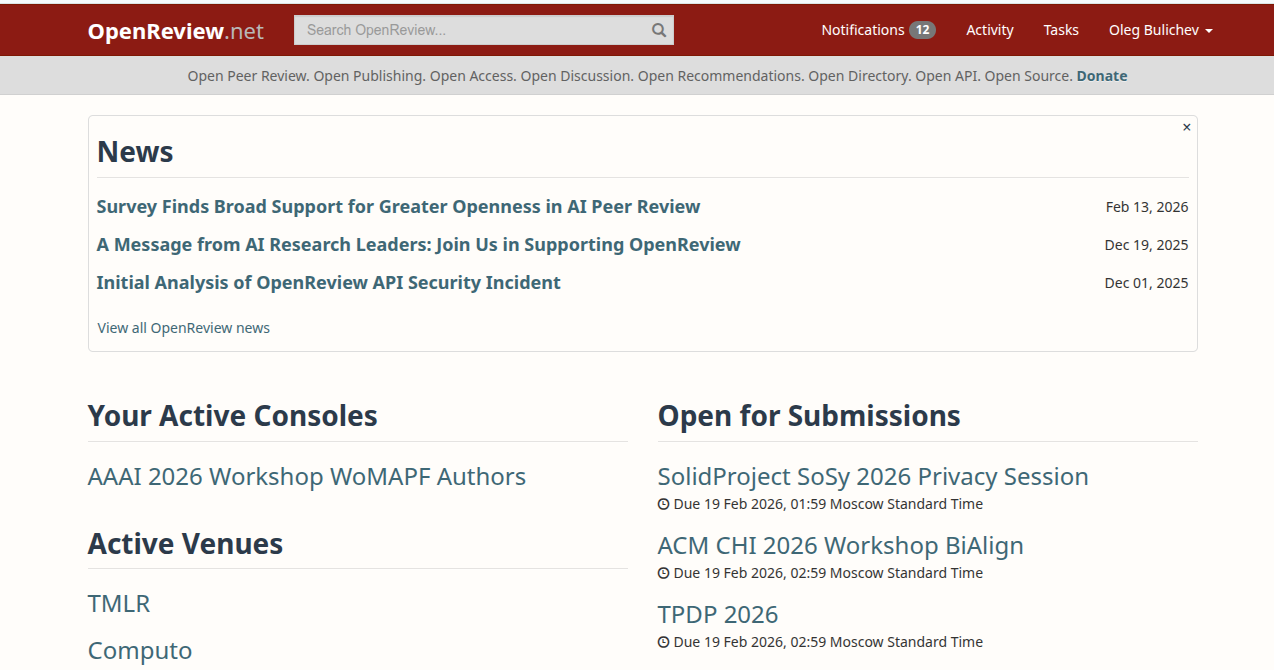
\includegraphics[height=6cm,width=1\textwidth,keepaspectratio]{openreview.png}
                        % \caption{caption_name}
                        \label{fig:openreview.png}
                    \end{figure}
                \end{minipage}
            \end{center}
        \end{column}
        \begin{column}{0.5\textwidth}
            \textbf{Microsoft CMT} (CVPR, ICCV)
            \begin{center}
                \begin{minipage}{0.9\textwidth}
                    \begin{figure}[H]
                        \centering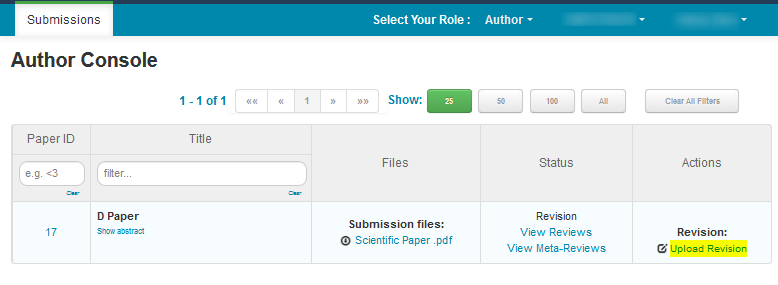
\includegraphics[height=6cm,width=1\textwidth,keepaspectratio]{microsoft.png}
                        % \caption{caption_name}
                        \label{fig:microsoft.png}
                    \end{figure}
                \end{minipage}
            \end{center}
        \end{column}
    \end{columns}
\end{frame}

\begin{frame}[t]{Workshops and Journals}
    \begin{columns}
        \begin{column}{0.5\textwidth}
            \textbf{Workshops:}
            \begin{itemize}
                \item Work in progress.
                \item Networking \& Feedback.
                \item Specific narrow topics.
                \item Less strict than main conference.
            \end{itemize}
        \end{column}
        \begin{column}{0.5\textwidth}
            \textbf{Journals:}
            \begin{itemize}
                \item Archival value.
                \item Longer review cycle (months/years).
                \item More detailed description.
            \end{itemize}
        \end{column}
    \end{columns}
\end{frame}

\begin{frame}[t]{Reference Materials}
    \begin{itemize}
        \item Conference websites (NeurIPS, ICLR, etc.) for requirements.
        \item \href{https://openreview.net/}{OpenReview.net}
        \item \href{https://cmt3.research.microsoft.com/}{Microsoft CMT}
    \end{itemize}
\end{frame}


\section{Searching for Literature}

\begin{frame}[t]{Searching for Literature}
    \begin{itemize}
        \item \textbf{Initial Search:}
        \begin{itemize}
            \item \textbf{Semantic Scholar:} standard for AI papers.
            \item \textbf{Asta (Ai2):} emerging tool.
            \item \textbf{Deep Research Agents:} perplexity, etc.
            \item \textbf{Scholar inbox:} AI-powered literature search.
        \end{itemize}
        \item Don't just rely on Google. Use academic-specific engines.
    \end{itemize}
\end{frame}

\begin{frame}{Apps for Literature Search}
\framesubtitle{}
    \vspace{-0.6cm}
    \begin{figure}[H]
        \begin{subfigure}[t]{0.49\textwidth}
            \centering
\includegraphics[height=6cm,width=1\textwidth,keepaspectratio]{asta.png}
            \caption*{Asta (AI2)}
        \end{subfigure}
        \begin{subfigure}[t]{0.49\textwidth}
            \centering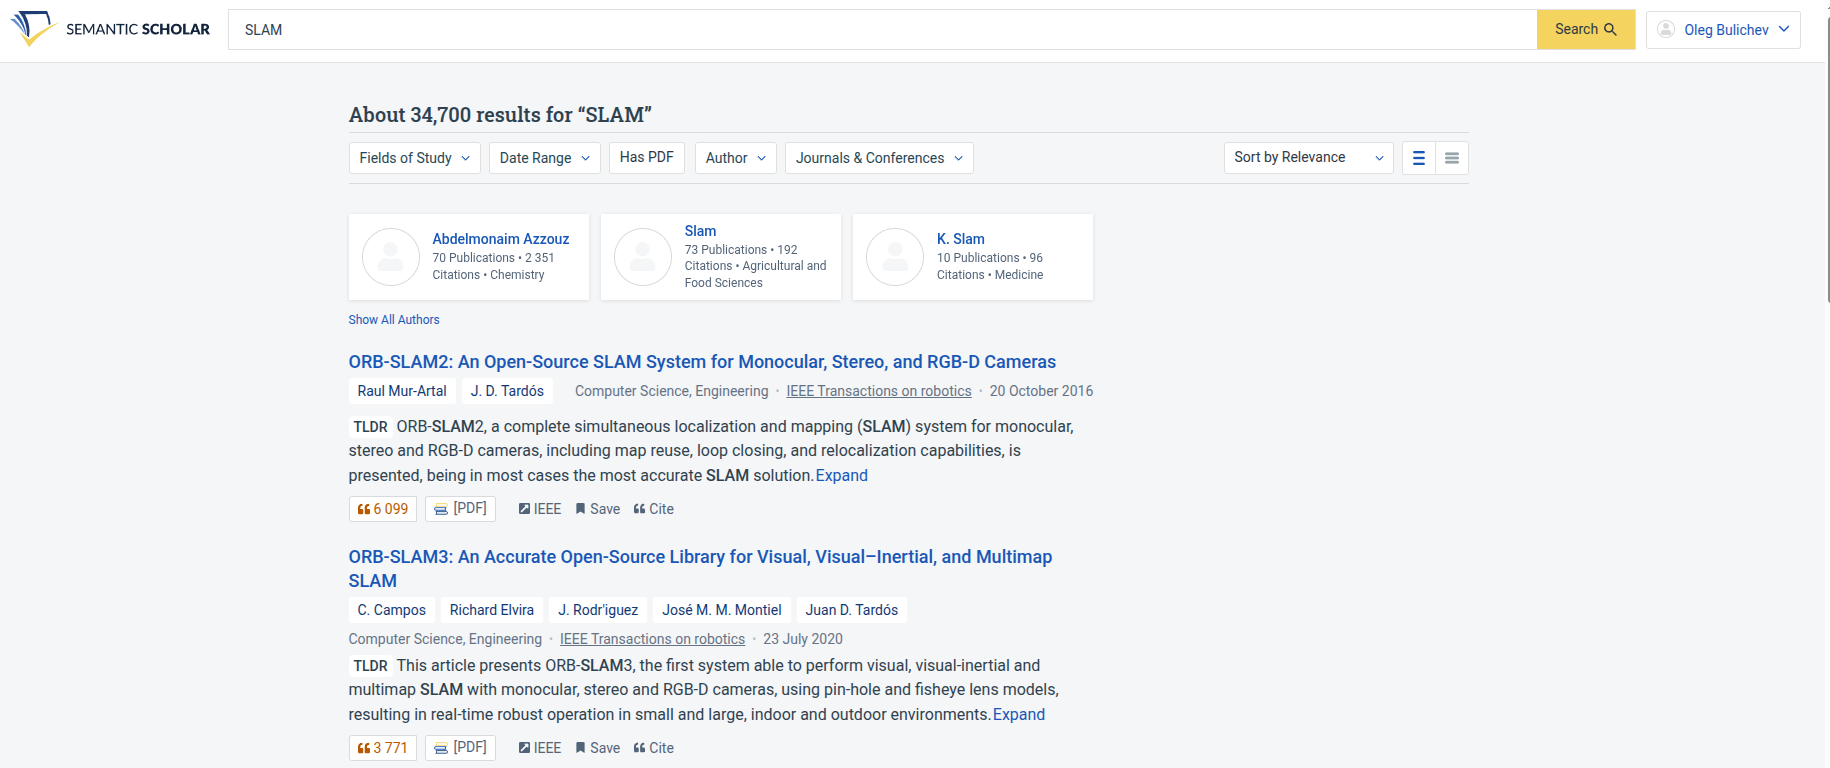
\includegraphics[height=6cm,width=1\textwidth,keepaspectratio]{semantic.png}
            \caption*{Semantic Scholar}
        \end{subfigure}
    \end{figure}
\end{frame}

\begin{frame}[t]{Publish or Perish (Application)}
    \begin{columns}
        \begin{column}{0.6\textwidth}
            \begin{itemize}
                \item \textbf{What is it?} A software program that retrieves and analyzes academic citations.
                \item \textbf{Key Features:}
                \begin{itemize}
                    \item Uses Google Scholar, Scopus, Web of Science.
                    \item Calculates h-index, g-index metrics.
                    \item Detailed citation analysis for authors or journals.
                    \item Helps identify "Must Read" classic papers by citation count.
                \end{itemize}
            \end{itemize}
        \end{column}
        \begin{column}{0.4\textwidth}
            \begin{figure}[H]
                \centering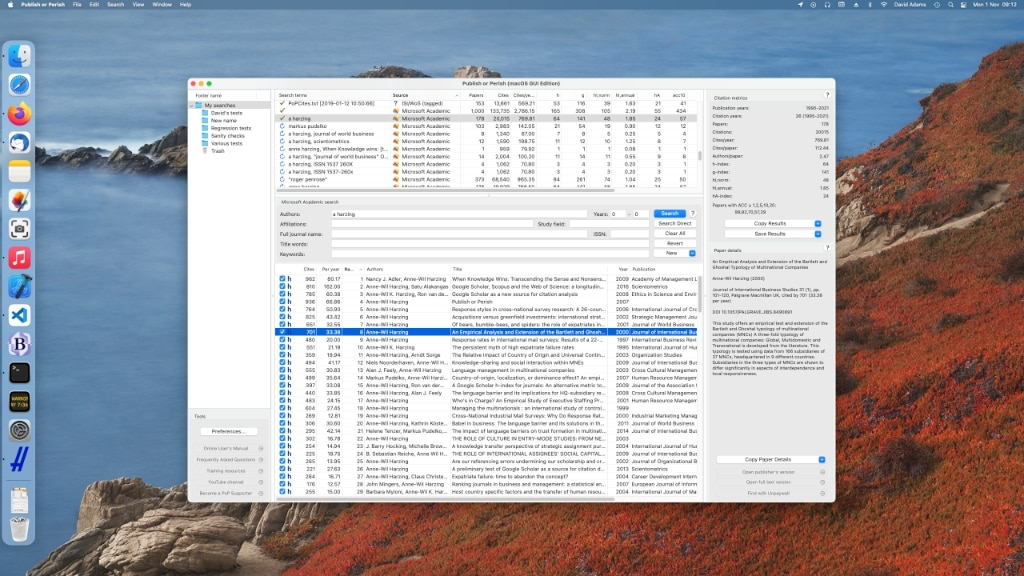
\includegraphics[height=6cm,width=1\textwidth,keepaspectratio]{pop8macos.jpg}
                \label{fig:pop8macos.jpg}
            \end{figure}
        \end{column}
    \end{columns}
\end{frame}


\begin{frame}[t]{Visualization of Connections}
    \begin{itemize}
        \item Build collections of papers.
        \item AI learns what you like and improves recommendations.
        \item Interactive visualization of author/paper networks.
        \item Infinite feed of related work.
    \end{itemize}
    \vspace{-0.4cm}
    \begin{figure}[H]
        \begin{subfigure}[t]{0.49\textwidth}
            \centering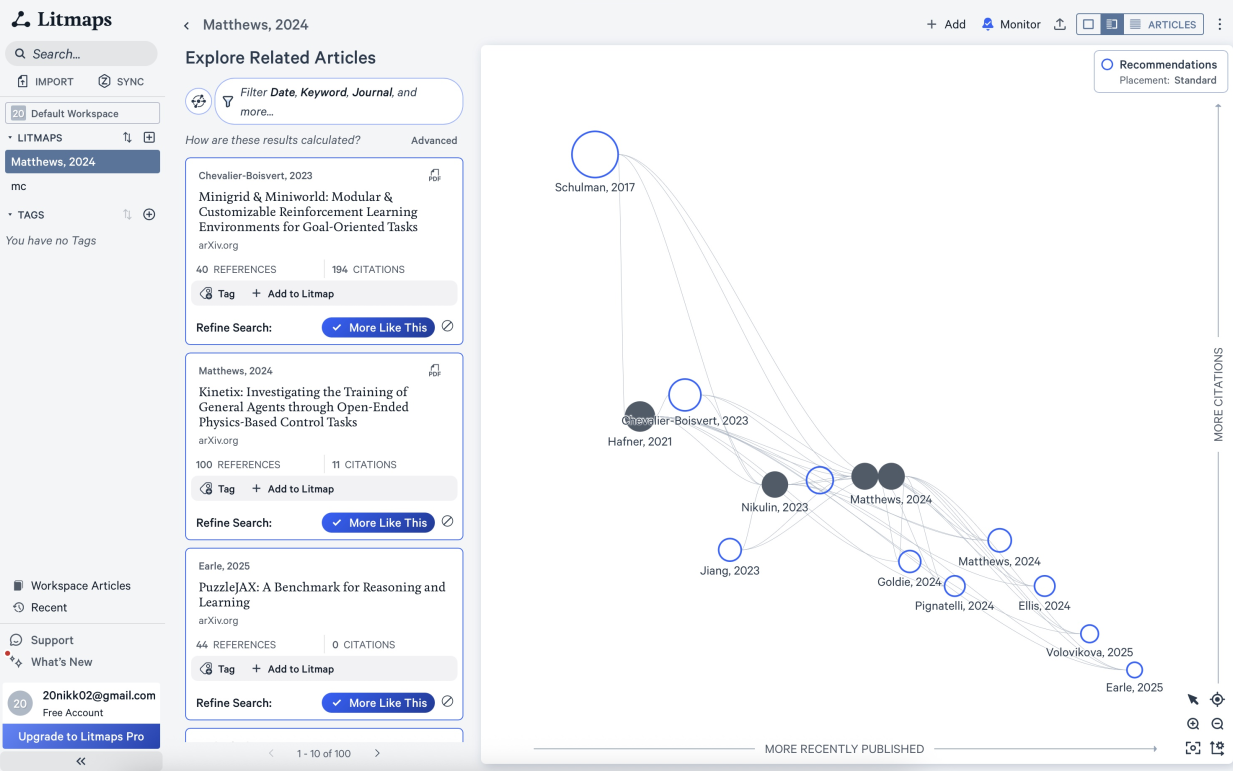
\includegraphics[height=3cm,width=1\textwidth,keepaspectratio]{litmap.png}
            \caption{Litmap}
            \label{fig:litmap.png}
        \end{subfigure}
        \begin{subfigure}[t]{0.49\textwidth}
            \centering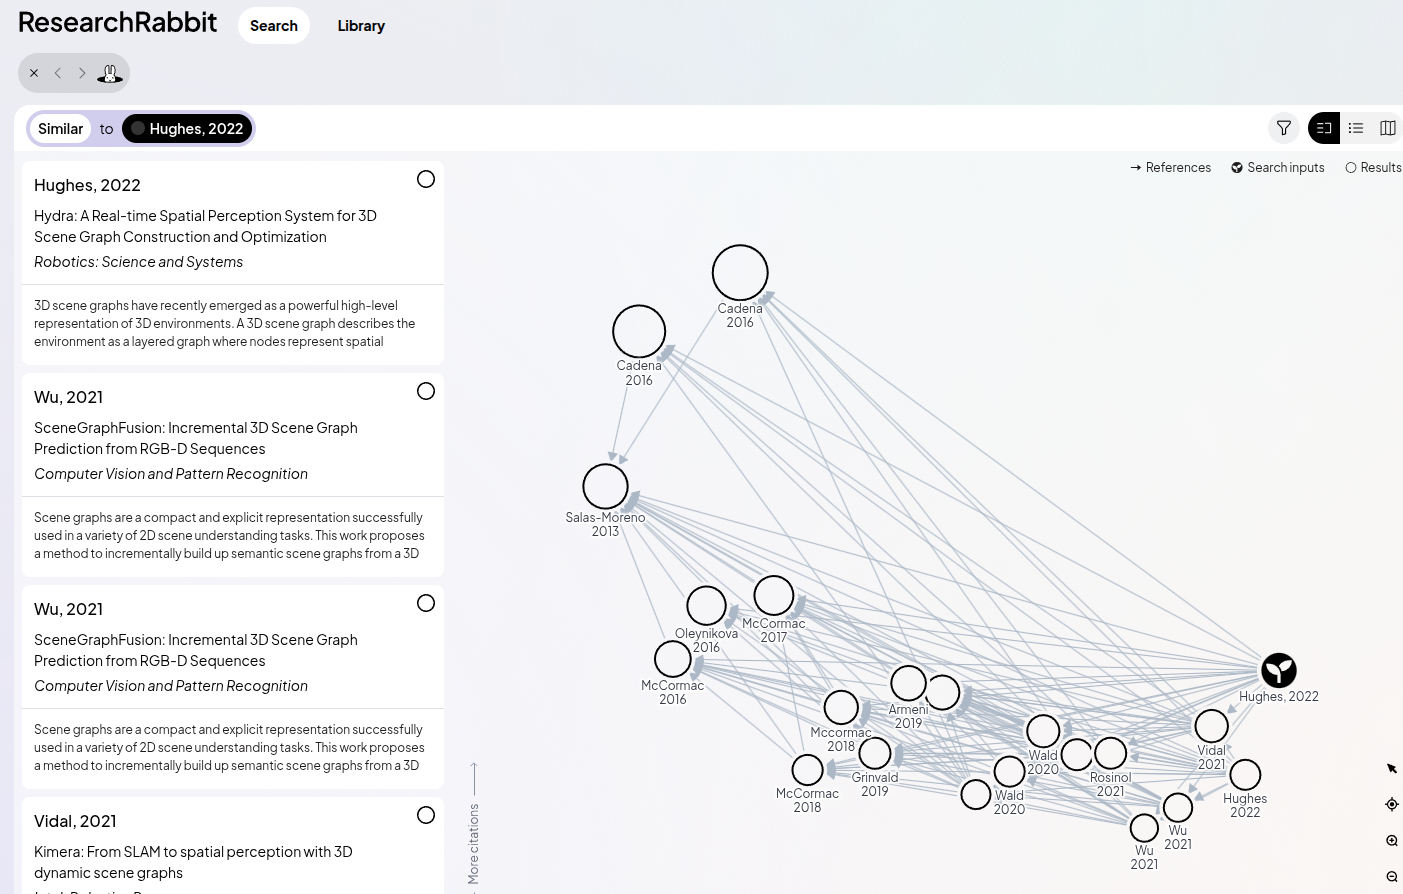
\includegraphics[height=3cm,width=1\textwidth,keepaspectratio]{researchrabbit.png}
            \caption{ResearchRabbit}
            \label{fig:researchrabbit.png}
        \end{subfigure}
    \end{figure}
\end{frame}

\begin{frame}[t]{Structing \& Information Extraction}
    \begin{itemize}
        \item \textbf{Elicit:} 
        \begin{itemize}
            \item "Research Assistant".
            \item Extract data from papers into a structured table.
            \item "What is the NMAE score for X?" across 10 papers.
        \end{itemize}
        \item \textbf{NotebookLM:} RAG system for synthesis.
    \end{itemize}
\end{frame}

\begin{frame}[t]{Elicit}
\framesubtitle{}
    \vspace{-0.6cm}
    \begin{figure}[H]
        \centering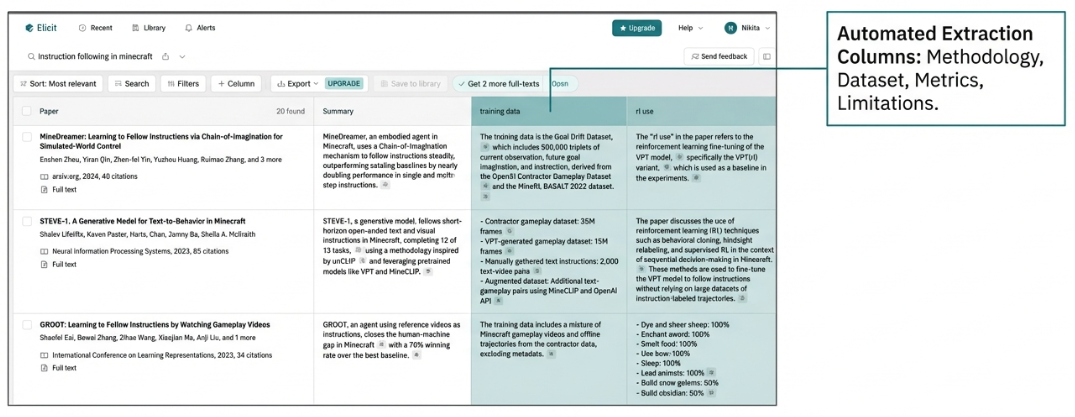
\includegraphics[height=6cm,width=1\textwidth,keepaspectratio]{elicit.png}
        \label{fig:elicit.png}
    \end{figure}
\end{frame}

\begin{frame}[t]{The MCP Pipeline (Advanced)}
    \textbf{Automation with MCP (Model Context Protocol):}
    \begin{enumerate}
        \item \textbf{Prompt:} Define strict search criteria.
        \item \textbf{AI Agent + Google Scholar MCP:} 
        \begin{itemize}
            \item Agent queries Scholar directly via MCP.
            \item Extracts Abstract \& DOI.
            \item Saves to Markdown.
        \end{itemize}
        \item \textbf{RAG Integration:} Feed md/pdfs to NotebookLM.
        \item \textbf{Generation:} Synthesize Technical Report.
    \end{enumerate}
\end{frame}


\begin{frame}[t]{Reference Materials}
    \begin{itemize}
        \item \href{https://smithery.ai/servers/JackKuo666/google-scholar-mcp-server}{Google Scholar MCP Server}
        \item \href{https://www.researchrabbit.ai/}{ResearchRabbit}
        \item \href{https://harzing.com/resources/publish-or-perish}{Publish or Perish App}
        \item \href{https://www.semanticscholar.org/}{Semantic Scholar}
        \item \href{https://elicit.com/}{Elicit.com}
        \item \href{https://www.litmaps.com/}{Litmaps}
        \item \href{https://www.perplexity.ai/}{Perplexity}
        \item \href{https://asta.allen.ai/}{Asta (Ai2)}
        \item \href{https://scholar-inbox.com/}{Scholar Inbox}
    \end{itemize}
\end{frame}


\section{Reference Management}

\begin{frame}[t]{Zotero: The Knowledge Hub}
    \begin{itemize}
        \item \textbf{Why Zotero 8?} Modern UI, native speed, built-in PDF reader.
        \item \textbf{Browser Connector:} One-click save (PDF + Metadata) from ArXiv, IEEE, etc.
        \item \textbf{Built-in Features:} 
        \begin{itemize}
            \item Automatic file renaming based on parent metadata.
            \item Extracting annotations to notes directly.
        \end{itemize}
        \item \textbf{Note Templates:} Configurable templates regarding your workflow.
    \end{itemize}
\end{frame}

\begin{frame}[t]{Essential Plugins}
    \begin{itemize}
        \item \textbf{Better BibTeX:} Generates stable Citation Keys (e.g., \texttt{bulichev2024ais}) for LaTeX/Overleaf.
        \item \textbf{Zotero SciPDF:} Automatically downloads PDFs via Sci-Hub if paywalled.
        \item \textbf{Better Notes:} Advanced knowledge management, markdown support, and bi-directional linking within Zotero.
    \end{itemize}
\end{frame}

\begin{frame}[t]{Teamwork \& BibTeX Generation}
    \begin{itemize}
        \item \textbf{Group Libraries:} 
        \begin{itemize}
            \item Share papers, PDFs, and notes with colleagues.
            \item Everyone sees the same PDF annotations.
        \end{itemize}
        \item \textbf{BibTeX Workflow:}
        \begin{itemize}
            \item Right-click Collection $\to$ Export Collection $\to$ Better BibTeX.
            \item Select "Keep updated" to auto-sync \texttt{.bib} file.
            \item \textbf{Overleaf:} Link the \texttt{.bib} file via URL or upload manually.
            \item \textbf{Citation Keys:} Ensure consistency (e.g., \texttt{[auth][year]}).
        \end{itemize}
    \end{itemize}
\end{frame}

\begin{frame}[t]{Obsidian Integration Workflow}
    \begin{itemize}
        \item \textbf{Goal:} Turn PDF highlights into permanent notes in your "Second Brain".
        \item \textbf{Tool:} \textit{Citations} plugin (Obsidian).
        \item \textbf{Process:}
        \begin{enumerate}
            \item Annotate PDF in Zotero.
            \item Use "Add Item Note from Annotations".
            \item Open Obsidian $\to$ "Insert Literature Note".
            \item Template auto-fills Title, Authors, Abstract, and your Zotero highlights.
        \end{enumerate}
    \end{itemize}
\end{frame}

\begin{frame}[t]{Zotero GUI}
\framesubtitle{}
    \vspace{-0.6cm}
    \begin{figure}[H]
        \centering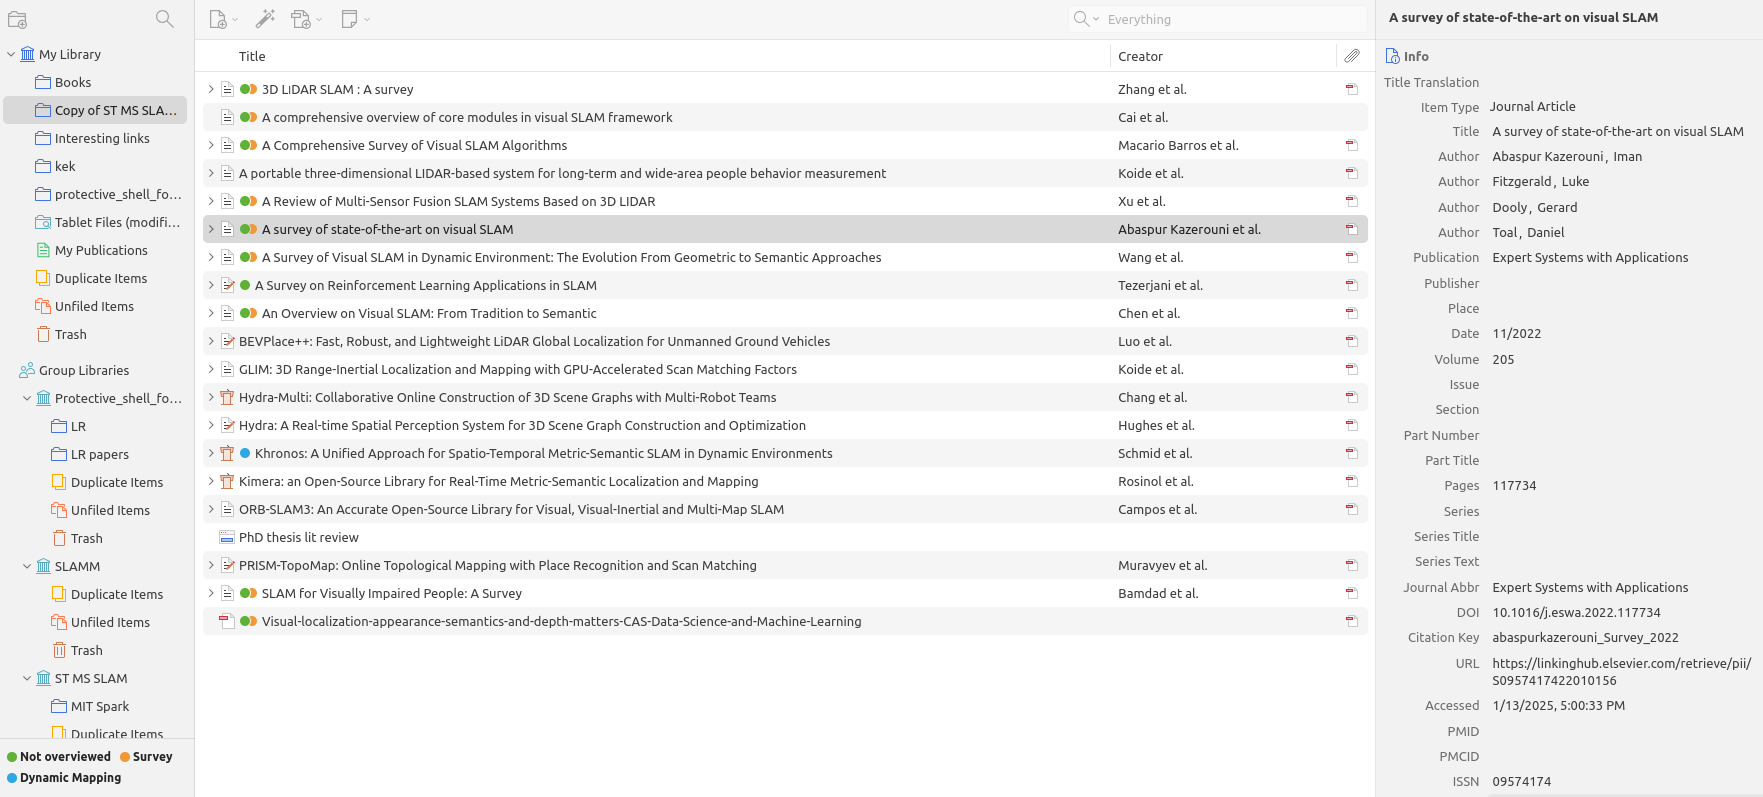
\includegraphics[height=6cm,width=1\textwidth,keepaspectratio]{zotero.png}
        \label{fig:zotero.png}
    \end{figure}
\end{frame}

\begin{frame}[t]{Reference Materials (Zotero)}
    \begin{itemize}
        \item \url{https://www.zotero.org/}
        \item \href{https://github.com/syt2/zotero-scipdf}{Zotero SciPDF (Zotero 7)}
        \item \href{https://github.com/windingwind/zotero-better-notes}{Better Notes Plugin}
        \item \href{https://retorque.re/zotero-better-bibtex/}{Better BibTeX Plugin}
    \end{itemize}
\end{frame}

\section{How to Read Papers}

\begin{frame}[t]{Reading Strategy with AI}
    \textbf{Goal:} Process information efficiently without losing depth.
    \vspace{0.5cm}
    \begin{itemize}
        \item Using AI assistants (LLMs) to interact with papers.
        \item Not just summarizing, but querying.
    \end{itemize}
\end{frame}

\begin{frame}[t]{Phase 1: Context \& Hallucinations}
    \begin{itemize}
        \item \textbf{Context Loading (RAG):} Use tools like NotebookLM or custom RAG pipelines to "chat" with the PDF.
        \item \textbf{Hallucination Check:} 
        \begin{itemize}
            \item Verify specific claims.
            \item Ask for page numbers/citations in the response.
            \item \textit{"Where exactly does the paper state X?"}
        \end{itemize}
    \end{itemize}
\end{frame}

\begin{frame}[t]{Phase 2: The Truth Seeker}
    \textbf{Generate Key Research Questions:}
    \begin{itemize}
        \item Instead of "Summarize this", ask:
        \begin{itemize}
            \item "What is the specific gap this paper fills?"
            \item "What are the limitations explicitly mentioned by authors?"
            \item "Compare method X with baseline Y based on the results tables."
        \end{itemize} 
    \end{itemize}
\end{frame}

\begin{frame}[t]{Phase 3: Deep Analysis}
    \begin{itemize}
        \item \textbf{Analyze Experiments:}
        \begin{itemize}
            \item Check experimental setup rigor.
            \item Metrics used (and why).
        \end{itemize}
        \item \textbf{Extract Insights:}
        \begin{itemize}
            \item What worked? What didn't?
            \item Why did they choose this architecture?
        \end{itemize}
    \end{itemize}
\end{frame}

\begin{frame}[t]{Secret Technique: Author Debates}
    \vspace*{-0.4cm}
    \begin{figure}[H]
        \centering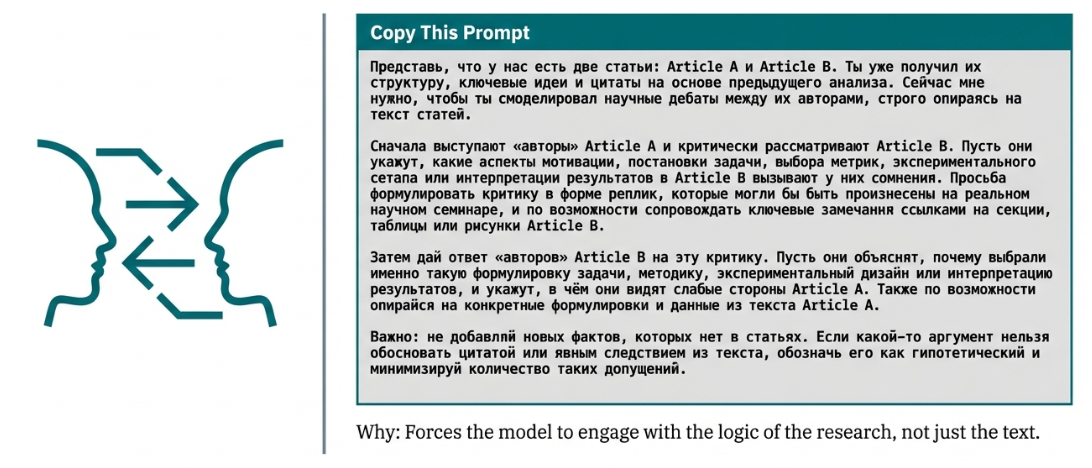
\includegraphics[height=6cm,width=1\textwidth,keepaspectratio]{author_debate.png}
        % \caption{caption_name}
        \label{fig:author_debate.png}
    \end{figure}
\end{frame}



\begin{frame}[t]{NotebookLM as a tool of avoiding hallucinations}
    \begin{center}
        \begin{minipage}{0.8\textwidth}
            \begin{figure}[H]
                \centering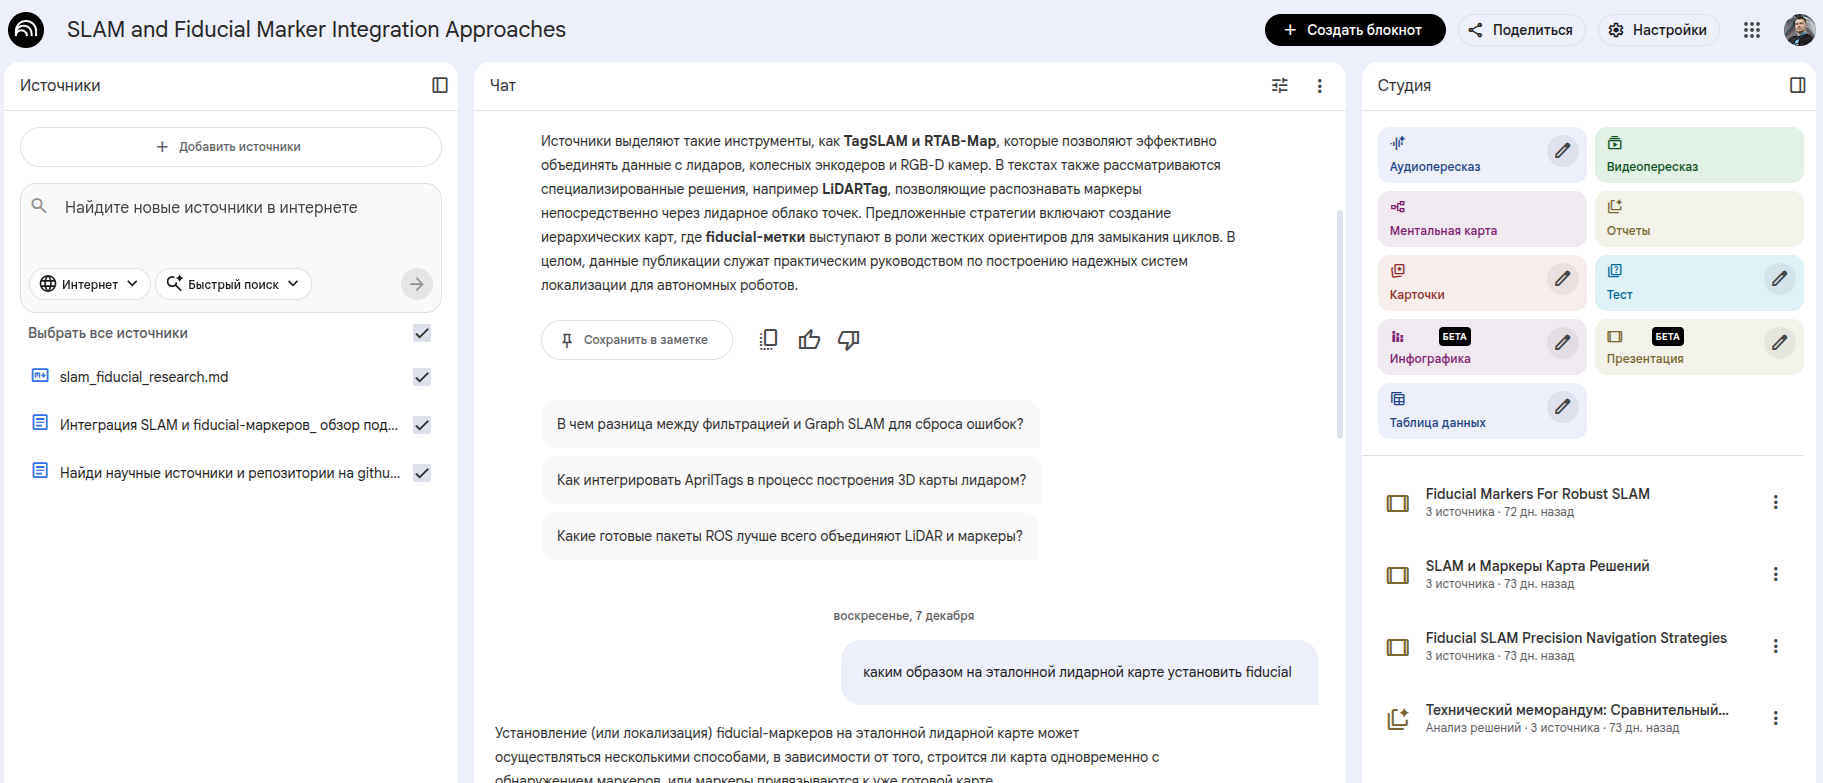
\includegraphics[height=6cm,width=1\textwidth,keepaspectratio]{notebooklm.png}
                % \caption{caption_name}
                \label{fig:notebooklm.png}
            \end{figure}
        \end{minipage}
    \end{center}
\end{frame}

\begin{frame}[t]{Your workflow}
\framesubtitle{}
    \vspace{-0.6cm}
    \begin{figure}[H]
        \centering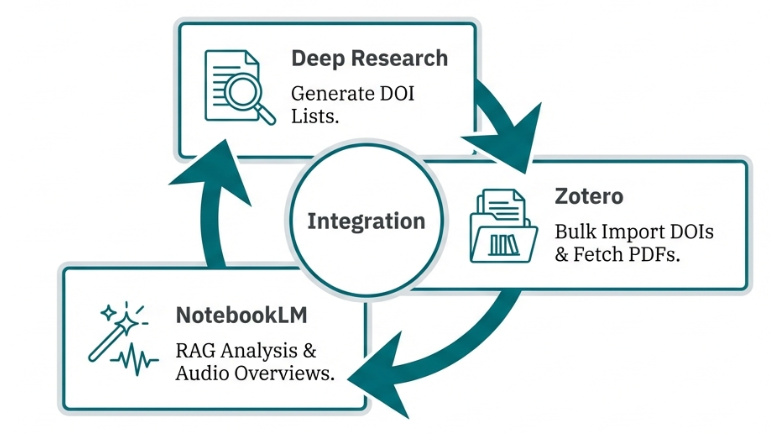
\includegraphics[height=6cm,width=1\textwidth,keepaspectratio]{power_user_workflow.png}
        \label{fig:power_user_workflow.png}
    \end{figure}
\end{frame}

\begin{frame}[t]{Reference Materials}
    \begin{itemize}
        \item \href{https://notebooklm.google/}{NotebookLM (Google).}
    \end{itemize}
\end{frame}


\section{Generating Core Part}

\begin{frame}[t]{From Plan to Text}
    \textbf{Method 1: Plan $\to$ Connected Text}
    \begin{itemize}
        \item Step 1: Create a detailed hierarchical plan (Chapters, Sections, Bullet points).
        \item Step 2: Use LLM to expand bullet points into paragraphs.
        \item \textbf{Crucial:} Freeze the structure. Don't let LLM wander.
    \end{itemize}
\end{frame}

\begin{frame}[t]{3 Levels of Text Work}
    To write clear and structured text, operate on three distinct levels:
    \vspace{0.5cm}
    \begin{enumerate}
        \item \textbf{Architecture Level:} The overall flow, chapter structure, and logic of the entire document.
        \item \textbf{Paragraph Level:} The logical unit of thought. Structure within a block.
        \item \textbf{Sentence Level:} Grammar, style, flow, vocabulary (Polishing).
    \end{enumerate}
\end{frame}

\begin{frame}[t]{Rules and tools for focusing}
\framesubtitle{}
    \vspace{-0.6cm}
    \begin{figure}[H]
        \centering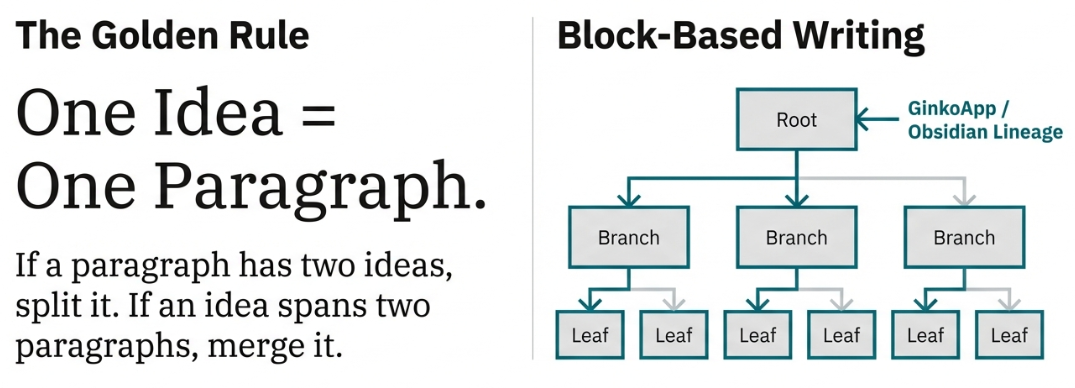
\includegraphics[height=6cm,width=1\textwidth,keepaspectratio]{ginko_boss.png}
        \label{fig:ginko_boss.png}
    \end{figure}
\end{frame}

\begin{frame}[t]{Tools for Block Writing}
    \begin{enumerate}
        \item \textbf{GinkoApp:} 
        \begin{itemize}
            \item Tree-based writing tool.
            \item Visualizes the hierarchy of thoughts.
        \end{itemize}
        \item \textbf{Lineage (Obsidian Plugin):}
        \begin{itemize}
            \item "The Gold Standard" for local workflow.
            \item Markdown based.
            \item Works inside Obsidian.
            \item Easy export to LaTeX/Pandoc.
        \end{itemize}
    \end{enumerate}
\end{frame}

\begin{frame}[t]{Block Writing in Action}
    \begin{columns}
        \begin{column}{0.5\textwidth}
            \textbf{GinkoApp Interface}
            \begin{center}
                \begin{minipage}{0.9\textwidth}
                    \begin{figure}[H]
                        \centering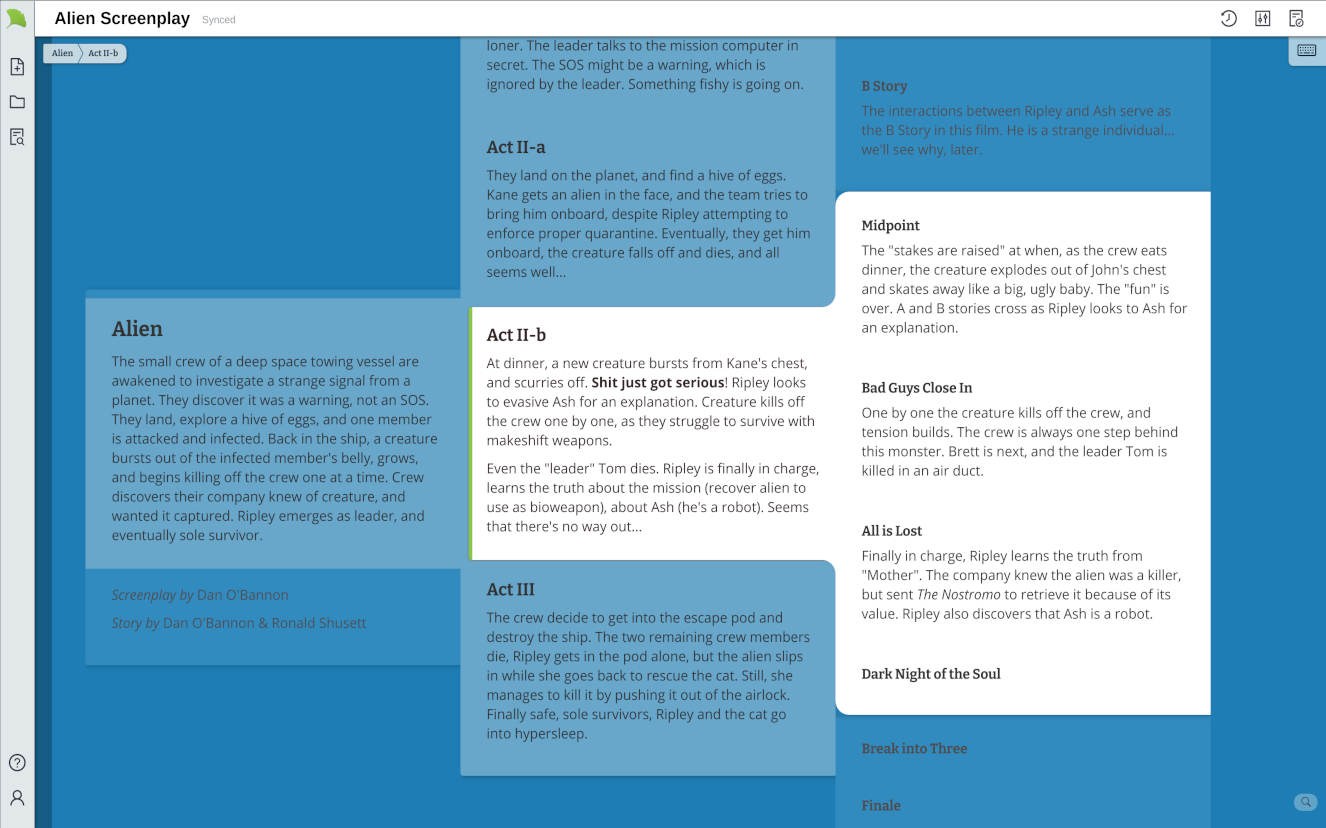
\includegraphics[height=6cm,width=1\textwidth,keepaspectratio]{ginko_site.png}
                        % \caption{caption_name}
                        \label{fig:ginko_site.png}
                    \end{figure}
                \end{minipage}
            \end{center}
        \end{column}
        \begin{column}{0.5\textwidth}
            \textbf{Lineage (Obsidian)}
            \begin{center}
                \begin{minipage}{0.9\textwidth}
                    \begin{figure}[H]
                        \centering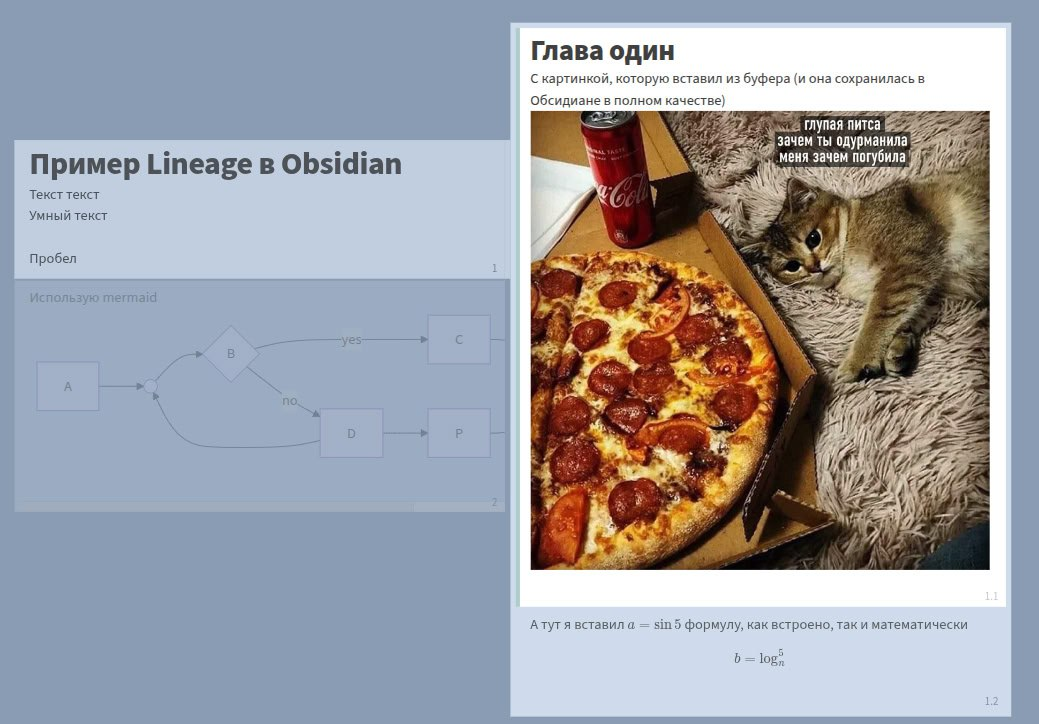
\includegraphics[height=6cm,width=1\textwidth,keepaspectratio]{lineage.jpg}
                        % \caption{caption_name}
                        \label{fig:lineage.jpg}
                    \end{figure}
                \end{minipage}
            \end{center}
        \end{column}
    \end{columns}
\end{frame}



\begin{frame}[t]{From Draft to Text}
    \textbf{Method 2: Draft $\to$ Connected Text}
    \begin{itemize}
        \item Step 1: Write a "Brain Dump" (rough draft, messy English/Russian).
        \item Step 2: Ask LLM to "Rewrite in Academic English, maintaining the flow".
        \item Better for preserving YOUR original ideas.
    \end{itemize}
\end{frame}

\begin{frame}[t]{Methodological Tricks}
    \begin{itemize}
        \item \textbf{Reduce Cognitive Load:} Don't ask for "Outcome + Formatting + Style" in one go. Split tasks.
        \item \textbf{Iterative Refinement:} 
        \begin{itemize}
            \item Draft $\to$ Critique $\to$ Edit.
        \end{itemize}
        \item \textbf{Context Management:} Provide definitions of symbols/terms to keep consistency.
    \end{itemize}
\end{frame}

\begin{frame}[t]{Meta-Prompting (For the Lazy)}
    \begin{itemize}
        \item Instead of writing the prompt yourself, ask a stronger model to write it.
        \item \textbf{Workflow:}
        \begin{enumerate}
            \item Tell DeepSeek/Opus: "I want to generate a section about X. Write a detailed System Prompt for GPT-4 to do this perfectly."
            \item Use the generated prompt.
        \end{enumerate}
    \end{itemize}
\end{frame}

\begin{frame}[t]{Image Generation for Papers}
    \begin{itemize}
        \item \textbf{Flux:} Good for diagrams and schematic illustrations.
        \item \textbf{DALL-E 3:} Integrated, follows instructions well, but can be "cartoony".
        \item \textbf{Use Case:} Visual Abstracts, concept diagrams.
        \item \textbf{Pro Tip:} Generate parts of diagram and assemble in Figma/TikZ.
    \end{itemize}
\end{frame}


\begin{frame}[t]{Reference Materials}
    \begin{itemize}
        \item \href{https://gingkowriter.com/}{GinkoApp}
        \item \href{https://github.com/ycnmhd/obsidian-lineage}{Obsidian Lineage Plugin}
        \item \href{https://www.youtube.com/watch?v=FdX2ovE4qV0}{
Using Gingko to Do the Single Method of Academic Writing}
        \item \href{https://blackforestlabs.ai/}{Flux (Black Forest Labs)}
        \item \href{https://chatgpt.com/}{DALL-E 3 (via ChatGPT)}
    \end{itemize}
\end{frame}


\section{Proofreading}

\begin{frame}[t]{Proofreading: Human vs AI}
    \begin{itemize}
        \item \textbf{AI Proofreading:} Good for grammar, flow, typo detection.
        \item \textbf{Human Proofreading:} Essential for logic, nuance, and "vibe".
        \item \textbf{Strategy:} AI Check $\to$ Human Edit $\to$ AI Final Polish.
        \item Use "Track Changes" mode in prompts ("Show me what you changed").
    \end{itemize}
\end{frame}

\begin{frame}[t]{Proofreading Interface Example (Grammarly)}
    \vspace*{-0.5cm}
\begin{figure}[H]
    \centering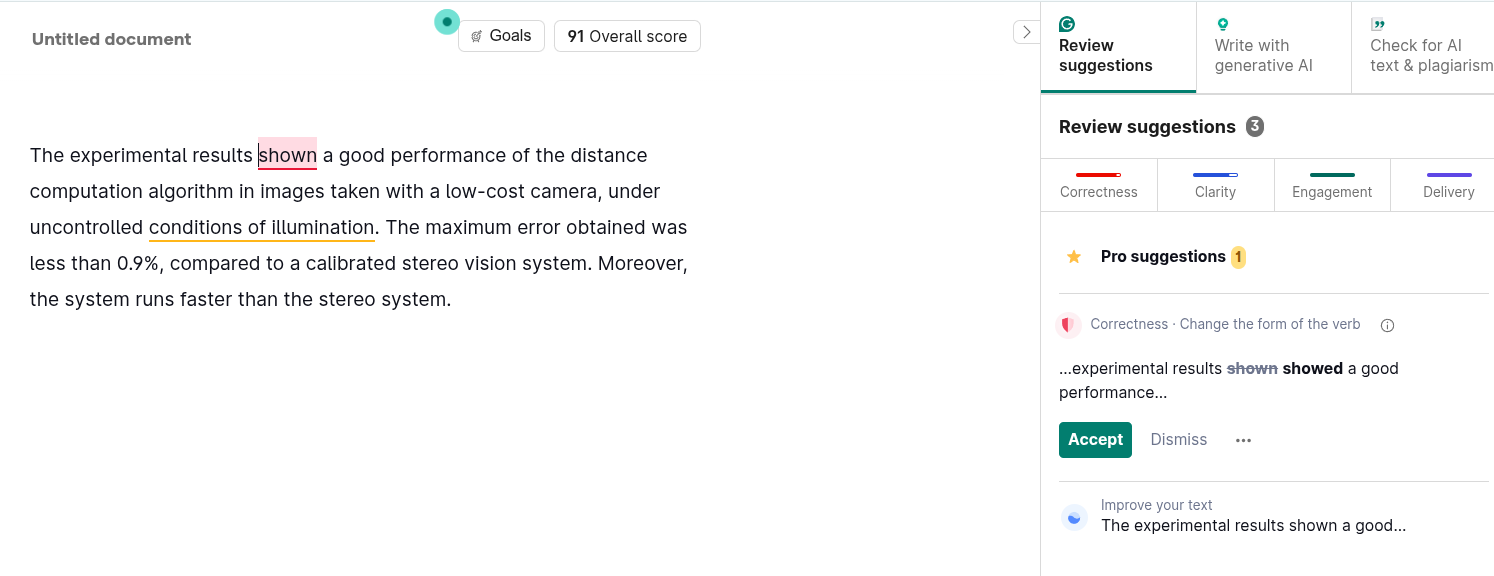
\includegraphics[height=6cm,width=1\textwidth,keepaspectratio]{grammarly.png}
    % \caption{caption_name}
    \label{fig:grammarly.png}
\end{figure}
\end{frame}

\begin{frame}[t]{Title Engineering}
    \begin{itemize}
        \item Title is the marketing of your paper.
        \item Use AI to generate 20 variations.
        \item Mix and Match: Combine the best parts.
        \item Keywords: Ensure SEO-friendly terms are in the title.
    \end{itemize}
\end{frame}

\begin{frame}[t]{Pre-submission Checklist}
    \begin{enumerate}
        \item Figures are readable in Black \& White?
        \item Captions explain the figure fully?
        \item Citations are correct?
        \item Formatting compliance?
        \item Spellcheck done?
    \end{enumerate}
\end{frame}


\section{Auto-review}

\begin{frame}[t]{AI as Reviewer}
    \textbf{Goal:} Get feedback BEFORE the actual reviewers destroy you.
    \vspace{0.5cm}
    \begin{itemize}
        \item \textbf{Tools:}
        \begin{itemize}
            \item \textbf{cspaper:} Specializes in AI conferences (NeurIPS, ICLR).
            \item \textbf{paperreview.ai}
        \end{itemize}
        \item Simulate the peer-review process.
    \end{itemize}
\end{frame}

\begin{frame}[t]{Structure of an AI Review}
    \begin{itemize}
        \item \textbf{Summary:} Does the AI understand your paper? (If not, rewrite).
        \item \textbf{Strengths \& Weaknesses:} Crucial feedback.
        \item \textbf{Questions:} What is unclear?
        \item \textbf{Rating:} (e.g., 1-10 scale).
        \item \textbf{Confidence:} (Low confidence = confusing paper).
    \end{itemize}
\end{frame}

\begin{frame}[t]{Warning: Limitations}
    \begin{itemize}
        \item \textbf{Missing Related Work:} AI often hallucinates papers here. Verification is mandatory.
        \item \textbf{Bias:} Models may prefer certain writing styles.
        \item \textbf{Use it for constructive critique, not for the score.}
    \end{itemize}
\end{frame}

\begin{frame}[t]{Automated Review Interface}
\vspace*{-0.4cm}
\begin{figure}[H]
    \centering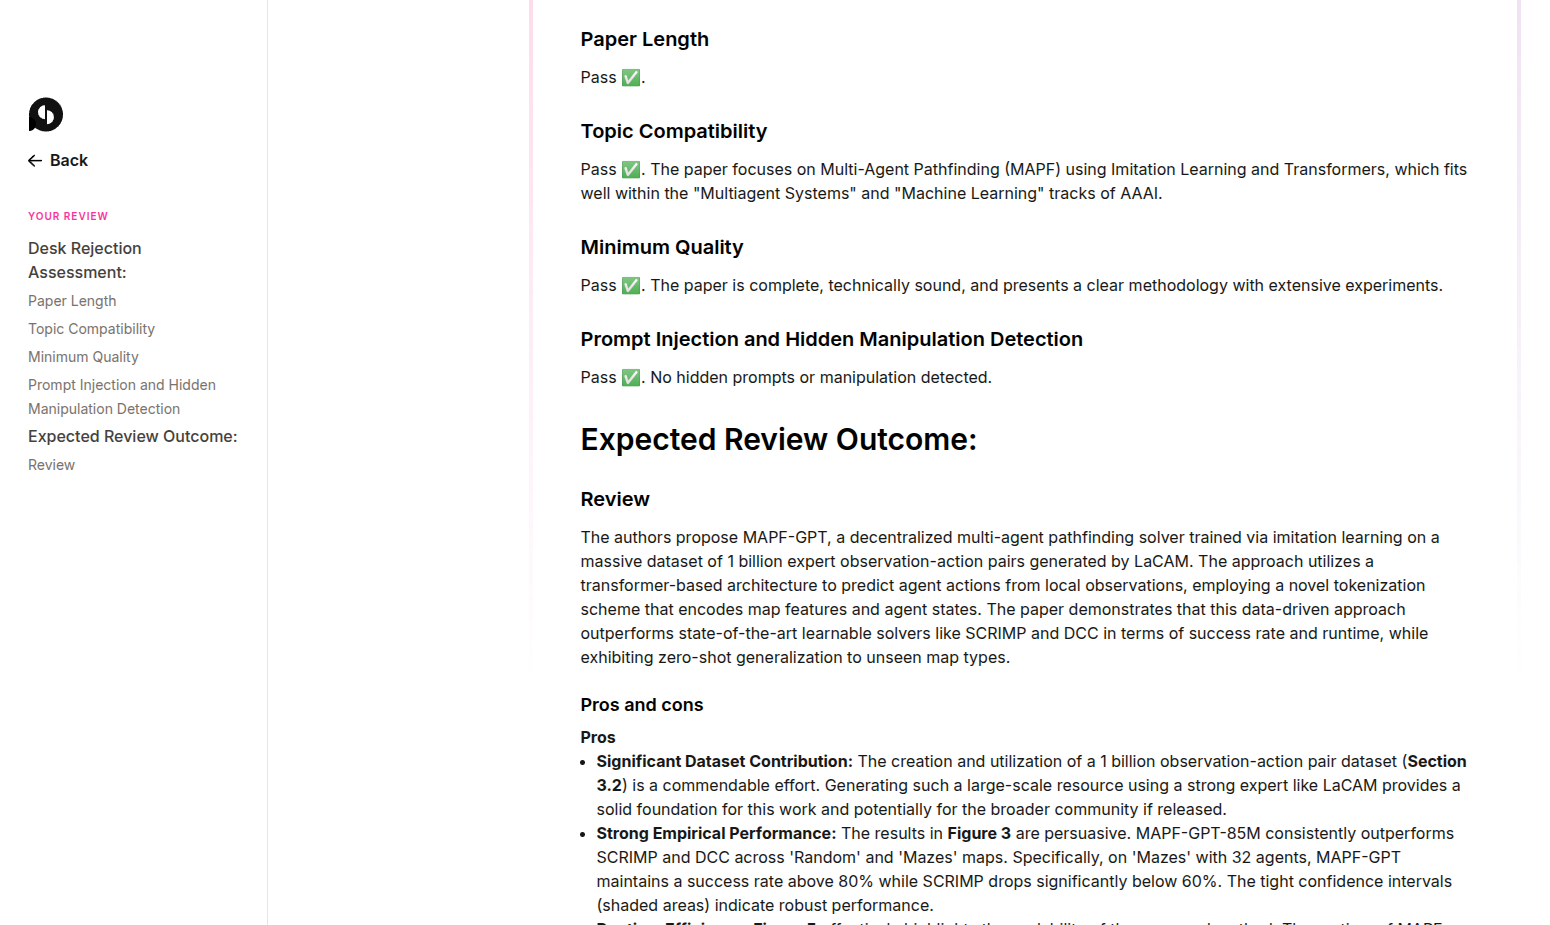
\includegraphics[height=6cm,width=1\textwidth,keepaspectratio]{cspaper.png}
    % \caption{caption_name}
    \label{fig:cspaper.png}
\end{figure}
\end{frame}

\begin{frame}[t]{Reference Materials}
    \begin{itemize}
        \item \url{https://cspaper.org/}
        \item \href{https://paperreview.ai/}{paperreview.ai}
    \end{itemize}
\end{frame}



\section{Detection of Generated Text}

\begin{frame}[t]{The Detection Problem}
    \begin{itemize}
        \item \textbf{ICLR Case:} Massive lazy reviewing with AI.
        \item 21\% of reviews were suspected to be AI-generated.
        \item \textbf{Why it matters:} Low effort reviews hurt science.
    \end{itemize}
\end{frame}

\begin{frame}[t]{Signs of Generated Text (Manual)}
    \begin{itemize}
        \item \textbf{Vocabulary:} Overuse of "delve", "underscore", "tapestry", "seamless", "landscape".
        \item \textbf{Structure:} Perfect, monotonous paragraph lengths.
        \item \textbf{Lack of Specifics:} Vague claims ("method is robust") without data ("method achieved 95\%").
    \end{itemize}
\end{frame}

\begin{frame}[t]{Technical Detection}
    \begin{itemize}
        \item \textbf{Unicode Artifacts:} AI might use weird symbols.
        \item \textbf{Services:}
        \begin{itemize}
            \item GPTZero, Pangram, Originality.ai.
        \end{itemize}
        \item \textbf{Problem:} High False Positive rate. 
        \item Good papers can be flagged as AI. Don't trust detectors 100\%.
    \end{itemize}
\end{frame}

\begin{frame}[t]{Reference Materials}
    \begin{itemize}
        \item \href{https://pangramlabs.com/}{Pangram Labs}
        \item \href{https://gptzero.me/}{GPTZero}
    \end{itemize}
\end{frame}

\begin{frame}[t]{}
\framesubtitle{}
    \begin{center}
        \Large AI is the accelerator. You are the driver. Keep your hands on the wheel.

    \end{center}
\begin{figure}[H]
    \centering
\includegraphics[height=5cm,width=1\textwidth,keepaspectratio]{auf.jpeg}
    % \caption{caption_name}
    \label{fig:auf.jpeg}
\end{figure}
\end{frame}

\fbckg{fibeamer/figs/last_page.png}
\frame[plain]{}

\end{document}